\documentclass[10pt]{article}
\usepackage{tmlr}
% Camera-ready: \usepackage[accepted]{tmlr}. Preprint (de-anonymized): \usepackage[preprint]{tmlr}.
\usepackage{booktabs}
\usepackage{array}
\usepackage{amsmath}
\usepackage{graphicx}
\usepackage{xcolor}
\usepackage{url}
\usepackage[hidelinks]{hyperref}
\newcommand{\qtN}{400}
\newcommand{\qtSizeFp}{3.8}
\newcommand{\qtAccEight}{91.75}
\newcommand{\qtSizeEight}{2.2}
\newcommand{\qtAccSix}{93.50}
\newcommand{\qtSizeSix}{1.7}
\newcommand{\qtDeltaSix}{+1.75}
\newcommand{\qtLostSix}{6}
\newcommand{\qtGainedSix}{13}
\newcommand{\qtPSix}{0.167}
\newcommand{\qtAccFive}{90.75}
\newcommand{\qtSizeFive}{1.5}
\newcommand{\qtDeltaFive}{-1.00}
\newcommand{\qtLostFive}{10}
\newcommand{\qtGainedFive}{6}
\newcommand{\qtPFive}{0.454}
\newcommand{\qtAccFour}{92.00}
\newcommand{\qtSizeFour}{1.3}
\newcommand{\qtDeltaFour}{+0.25}
\newcommand{\qtLostFour}{13}
\newcommand{\qtGainedFour}{14}
\newcommand{\qtPFour}{1.000}
\newcommand{\qtAccThree}{87.00}
\newcommand{\qtSizeThree}{1.1}
\newcommand{\qtDeltaThree}{-4.75}
\newcommand{\qtLostThree}{30}
\newcommand{\qtGainedThree}{11}
\newcommand{\qtPThree}{0.004}
\newcommand{\qtSizeRatioFour}{59}
\newcommand{\qtCompressFour}{34}
\newcommand{\qtRepRunsEight}{3}
\newcommand{\qtRepMeanEight}{91.58}
\newcommand{\qtRepRangeEight}{0.25}
\newcommand{\qtRepListEight}{91.75, 91.50, 91.50}
\newcommand{\qtRepFlipsMaxEight}{1}
\newcommand{\qtRepRunsFour}{3}
\newcommand{\qtRepMeanFour}{91.83}
\newcommand{\qtRepRangeFour}{0.50}
\newcommand{\qtRepListFour}{92.00, 91.50, 92.00}
\newcommand{\qtRepFlipsMaxFour}{4}
\newcommand{\qtMaxRepRange}{0.50}
\newcommand{\qtCliffOverNoise}{10}
\newcommand{\qtRungsCount}{5}
\newcommand{\qtRunsTotal}{9}
\newcommand{\qtMacTg}{35}
\newcommand{\qtMacPp}{650}
\newcommand{\qtGcpTg}{22.0}
\newcommand{\qtGcpPp}{109.6}

\newcommand{\blocked}[1]{\textcolor{red}{\textbf{[BLOCKED, pending measurement: }#1\textbf{]}}}
\newcommand{\bfcl}{BFCL}
\newcommand{\qm}{Qwen3-1.7B}

\title{Where Post-Training Quantization Breaks Agentic Tool Calling: A k-Quant Ladder on Qwen3 and Llama}

% Hidden by tmlr.sty unless [accepted] or [preprint] is passed.
\author{\name Akshay Kumar \email akumar8@mt.iitr.ac.in \\
      \addr Independent Researcher, Seattle, WA, USA}

\def\month{MM}
\def\year{YYYY}
\def\openreview{\url{https://openreview.net/forum?id=XXXX}}

\begin{document}
\maketitle

\begin{abstract}
Models reach laptops through post-training quantization, and the format that ships is the llama.cpp k-quant. Its cost has been measured on prose, knowledge and reasoning, never on what an agent does, which is emit a function call that a program executes. We build a controlled ladder, five k-quant formats from one FP16 source, and score each rung on the Berkeley Function Calling Leaderboard by deterministic syntax-tree matching, with no model judging another anywhere in the pipeline. We pre-registered the intuition that a function signature, having no slack, would break at a higher bit-width than free-form text. It does not. On \qm{} tool calling is flat from Q8\_0 through Q4\_K\_M and loses \qtDropThree{} points at Q3\_K\_M, about \qtCliffOverNoise{} times the run-to-run noise we measure by re-running identical weights. On the same weights, free-form mathematics loses \qtGsmDropThree{} points at the same rung, because \qtGsmTruncPctThree{}\% of generations run out of a 4{,}096-token budget still inside the chain of thought. Tool calls are short enough that this run-away never has room to happen, which is why the schema survives. The cliff is absent on Qwen3-8B and Qwen3-14B. A second family does not follow the pattern: Llama-3.2-3B already loses \qtDropLlamaThreeBFour{} points at Q4\_K\_M, and Llama-3.1-8B scores \qtDropLlamaEightBThree{} points higher at Q3\_K\_M than at Q8\_0 under the strict checker because its full-precision weights quote numeric arguments as strings; a checker that coerces such strings restores the expected order and a \qtLlamaEightBCoercedDropThree{}-point loss at three bits. A fair answer extractor changes the free-form numbers by at most \qtGsmGapMax{} points, and a logit penalty on overthinking markers has no measurable effect on tool calling at either rung. On Qwen3, four-bit quantization is safe and three-bit is not; on Llama the floor moves with the model, so the bit-width an agent can tolerate has to be measured rather than assumed, and the damage quantization does to long reasoning does not carry over to the tool call.
\end{abstract}

\section{Introduction}

Language models reach laptops by being compressed. The weights are stored in fewer bits than they were trained in, and the file shrinks accordingly. The full-precision file for \qm{} is \qtSizeFp{}\,GB; the version most people would actually run, Q4\_K\_M, is \qtSizeFour{}\,GB, about \qtCompressFour{}\% of it. That compression is post-training quantization \citep{dettmers2022int8,gptq2023,awq2024}, and the format nearly everyone uses on a laptop is the family of llama.cpp k-quants \citep{llamacpp}, because that is what Ollama and every desktop front end serve. Four bits is where the scaling analysis says the trade-off is best \citep{dettmers2023case,kumar2024precision}, and it is the default most front ends pull. Lower bit-widths are pursued for throughput as well as size, although \citet{malekar2025amdahl} show that those gains are capped by whatever part of the model stays in higher precision.

The cost of that compression has been measured with care, but on the wrong tasks for one growing use. Broad evaluations cover language modelling, classification, knowledge, dialogue, long context and trustworthiness across many families \citep{jin2024comprehensive,li2024evaluating}, multilingual degradation has its own study \citep{marchisio2024multilingual}, long-context inputs lose up to 59\% under four-bit methods \citep{mekala2025longcontext}, and reasoning models have been quantized and scored on mathematics and code \citep{liu2025quanthurts}. \citet{kurt2026quant} quantizes Llama-3.1-8B-Instruct into thirteen GGUF formats and scores each on GSM8K, HellaSwag, IFEval, MMLU, TruthfulQA and perplexity. \citet{lotfi2026overthink} measure five reasoning models under GPTQ, AWQ and FlatQuant on mathematics, code and science questions and find accuracy falling as chain-of-thought inflates. Every task in both papers is free-form or multiple choice, and none of them involves emitting a function call, which is the output an agent actually produces.

An agent calls tools \citep{patil2023gorilla,qin2023toolllm,yao2024taubench}. It emits a function name and a set of typed arguments that a program will execute. That output either parses against the schema or it does not, with no partial credit and no reader to accept an approximate answer. Our starting intuition was that a function signature has none of the slack prose has, and that compression should therefore break tool calling at a higher bit-width than free-form accuracy. We pre-registered this as our first hypothesis before running anything.

We build a controlled ladder, five k-quant formats produced from one FP16 source, and score each rung on the Berkeley Function Calling Leaderboard \citep{bfcl2025}, which compares a model's call to a reference by deterministic abstract-syntax-tree matching. No model judges another model anywhere in the pipeline. We then run the same weights on a free-form control so that the two floors can be compared on identical parameters.

For \qm{} the answer is the reverse of the one we expected. Tool-calling accuracy is flat from Q8\_0 through Q4\_K\_M and falls by \qtDropThree{} points at Q3\_K\_M, roughly \qtCliffOverNoise{} times the run-to-run noise of the instrument. On the same weights free-form mathematics falls by \qtGsmDropThree{} points at the same rung. Both floors sit between four and three bits, but the drop in tool calling is about an eighth of the drop in mathematics. The difference comes down to output length. At three bits the model's chain of thought \citep{wei2022cot} grows until \qtGsmTruncPctThree{}\% of math generations use up their token budget before reaching an answer. A tool call is a median of \qtToolNgenMedThree{} tokens, so the same weights never get the chance to wander. On Qwen3-8B and Qwen3-14B there is no cliff at any rung. On a second family the picture changes: Llama-3.2-3B already loses at four bits, and Llama-3.1-8B scores higher on tool calling when compressed, for a reason that has nothing to do with capability (\S\ref{sec:family}).

\paragraph{Contributions.} A controlled k-quant ladder for agentic tool calling, built from one source per model so that only the weights change between rungs (\S\ref{sec:method}). A reproducibility measurement that most quantization papers omit: the same weights run three times, which bounds what a ladder difference can mean (\S\ref{sec:repro}). The floor for \qm{}, located between Q4\_K\_M and Q3\_K\_M by paired testing (\S\ref{sec:ladder}). The free-form comparison on identical weights, which reverses H1 and locates the mechanism in chain-of-thought length rather than in the schema (\S\ref{sec:freeform}). The same measurement at 8B and 14B, where the cliff disappears (\S\ref{sec:models}). The same ladder on a second family, Llama-3.2-3B and Llama-3.1-8B, where the floor sits above four bits for the 3B model and where compression raises the 8B model's schema score by changing an argument-typing habit (\S\ref{sec:family}). A deployment table for a question practitioners currently answer by guessing.

\section{Related work}

\paragraph{Quantization evaluated on free-form tasks.} The broad evaluations of post-training quantization score many model families on language modelling, multiple-choice knowledge, dialogue, long-context and trustworthiness tasks \citep{jin2024comprehensive,li2024evaluating}; a full-text search of both finds no tool-calling or function-calling benchmark. \citet{liu2025quanthurts} quantize the DeepSeek-R1-distilled and QwQ reasoning models and find mathematics and code degrading under aggressive weight and KV-cache quantization, again on free-form tasks. \citet{kurt2026quant} is the closest work and the one this paper extends. One model, thirteen llama.cpp formats from Q3\_K\_S to Q8\_0 against FP16, six free-form or multiple-choice benchmarks, plus throughput and size. A full-text read finds no tool-calling, function-calling, agentic, structured-output or schema-compliance evaluation, and the conclusion asks for exactly what we add: additional model families and sizes under the same protocol. \citet{lotfi2026overthink} take a different axis, in the line of work on overthinking in reasoning models \citep{chen2024overthinking,sui2025stop}. Under GPTQ \citep{gptq2023}, AWQ \citep{awq2024} and FlatQuant, five reasoning models lose accuracy while emitting longer chains of thought, and in up to 52\% of failures the correct answer appears mid-trace without being committed to. Two details matter for the comparison. Their compression methods are research methods rather than the k-quants that ship to laptops, and their failure categorisation, including the overthinking class, relies on GPT-5 as a judge, whereas our pipeline contains none.

\paragraph{Tool-calling evaluation.} Gorilla \citep{patil2023gorilla} and ToolLLM \citep{qin2023toolllm} established API calling as a benchmark task, and $\tau$-bench \citep{yao2024taubench} extends it to multi-turn agent-user interaction. \bfcl{} \citep{bfcl2025} scores a model's function call against a reference by abstract-syntax-tree matching over the function name, argument names, types and values, across single, multiple and parallel calls, an irrelevance category where no call is correct, and multi-turn trajectories. Because the matcher is deterministic, the same generation always receives the same verdict, which is what lets a ladder difference be attributed to the weights rather than to the scorer. \citet{dondeti2026toolguard} study the same class of small models on consumer hardware from the safety side, scoring adversarial tool calls from seven models between 1B and 4B parameters with a deterministic would-dispatch rule; this paper is the accuracy side of the same deployment.

\paragraph{The gap.} Quantization has been scored on prose, knowledge, instruction following and reasoning, both for research compression methods and for the deployed one. It has not been scored on tool calling under either, and that is what we measure.

\section{Method}
\label{sec:method}

\paragraph{Pre-registration.} Hypotheses and thresholds were fixed on 18 September 2026 before the first grid run and are in \texttt{paper/preregistration.md}. Two full-text summaries were appended to that file during the first rung as documentation; no hypothesis or threshold changed after runs began.

\paragraph{The ladder.} Every rung is produced from a single FP16 GGUF of \qm{} \citep{qwen3} with \texttt{llama-quantize}, so the rungs differ in weights and in nothing else. The formats are a subset of the ladder in \citet{kurt2026quant}, chosen to span the range at one rung per bit-width: Q8\_0, Q6\_K, Q5\_K\_M, Q4\_K\_M and Q3\_K\_M. Ollama's library publishes only three of these for this model, which is why the ladder is built rather than pulled.

\paragraph{Serving.} Each rung is served by \texttt{llama-server} with full Metal offload under a fixed model alias, so the harness sends identical requests to every rung. The single-call ladder and the repeats use four slots and an 8{,}192-token context; the free-form control, the larger models and the multi-turn runs use 32{,}768, because reasoning traces overflowed the smaller context; the 16{,}384-token budget re-run uses 65{,}536 with two slots. Generation is at temperature 0.001. Measured throughput is about \qtMacTg{} tokens per second per slot and \qtMacPp{} tokens per second of prompt evaluation on an Apple M1 Max.

\paragraph{Scoring.} \bfcl{} v4, \texttt{simple\_python} category, \qtN{} questions, deterministic AST matching. Differences between rungs are tested pairwise on the same \qtN{} questions with McNemar's exact test \citep{mcnemar1947}, which uses only the discordant pairs and is the appropriate test when two conditions are scored on identical items.

\paragraph{Reproducibility control.} Two rungs, Q8\_0 and Q4\_K\_M, were run three times each with identical weights and settings. This gives the run-to-run variation of the instrument, which is needed before any difference between rungs can be read as a difference between weights.

\paragraph{Free-form control.} The same five weight files answer 400 GSM8K test questions \citep{gsm8k2021}, drawn at seed 42, through the same server under the same alias, with a 4{,}096-token completion budget. Every generation is logged in full so that scoring under a different extractor is a re-read rather than a re-run. Two extractors were fixed before any rung was scored. Strict accepts an explicit commitment in any of three forms: ``The answer is $N$'', ``\#\#\#\# $N$'', or $\backslash$boxed$\{N\}$. Lenient takes the last number in the visible answer. We record that our first strict rule accepted only the first form and would have scored 21 of the first 59 generations wrong for writing the answer in a box; that rule was a strawman and was replaced before scoring, and the gap it would have produced is not reported anywhere in this paper.

\paragraph{Larger models and a second family.} Qwen3-8B, same three rungs Q8\_0, Q4\_K\_M and Q3\_K\_M from its own FP16 source, on the first \qtNEightB{} questions of the same category in file order, and Qwen3-14B under the identical protocol. Llama-3.2-3B-Instruct and Llama-3.1-8B-Instruct \citep{llama3}, from their own FP16 sources, at the same three rungs, on the same \qtNEightB{} questions and the same 400 GSM8K questions with the same prompt and budget. Both Llama models are instruction-tuned rather than reasoning-tuned, which is deliberate: it separates what the ladder does to a tool call from what it does to a chain of thought. Llama-3.1-8B-Instruct is also the model \citet{kurt2026quant} quantized, so the two ladders meet on one model.

\paragraph{Overthinking penalty.} \citet{lotfi2026overthink} report that a fixed logit penalty on a curated list of overthinking markers cuts chain-of-thought length by 12 to 23\% while preserving accuracy. We apply a fixed penalty of $-2.0$ to the eight Qwen3 tokens for \emph{wait}, \emph{but}, \emph{alternatively} and \emph{hmm} in both capitalisations, at the server, and re-run the \qm{} ladder at Q4\_K\_M and Q3\_K\_M. This approximates their method with a single fixed $\lambda$ rather than their tuned value.

\section{Results}

\subsection{The instrument is reproducible}
\label{sec:repro}

Table~\ref{tab:repeats} gives the same weights run three times. Q8\_0 moved by \qtRepRangeEight{} points across three runs and Q4\_K\_M by \qtRepRangeFour{}. At the level of individual questions, at most \qtRepFlipsMaxEight{} of \qtN{} verdicts changed between two Q8\_0 runs and at most \qtRepFlipsMaxFour{} between two Q4\_K\_M runs. The instrument is close to deterministic, so any difference between rungs larger than about \qtMaxRepRange{} points can be attributed to the weights rather than to run-to-run variation.

\begin{table}[t]
\centering\small
\begin{tabular}{@{}llrr@{}}
\toprule
Rung & Accuracy per run & Range (pp) & Max per-question flips \\
\midrule
Q8\_0 & 91.75, 91.50, 91.50 & 0.25 & 1 of 400 \\
Q4\_K\_M & 92.00, 91.50, 92.00 & 0.50 & 4 of 400 \\
\bottomrule
\end{tabular}

\caption{Run-to-run variation with identical weights and settings, \texttt{simple\_python}, $n=\qtN{}$.}
\label{tab:repeats}
\end{table}

\subsection{Flat to four bits, a cliff at three}
\label{sec:ladder}

Table~\ref{tab:ladder} is the ladder. From Q8\_0 down to Q4\_K\_M the accuracy sits in a band of under three points and no rung differs from Q8\_0 at any conventional level: Q4\_K\_M is at \qtAccFour{}\% against Q8\_0's \qtAccEight{}\%, a difference of \qtDeltaFour{} points with a McNemar $p$ of \qtPFour{}, while being \qtSizeRatioFour{}\% of the file size. Q6\_K scores above Q8\_0 and Q5\_K\_M below it, and neither difference survives paired testing, so the apparent non-monotonicity in the raw numbers is within the instrument's noise.

Q3\_K\_M is a different case. It loses \qtLostThree{} questions that Q8\_0 gets right and recovers \qtGainedThree{}, a net loss of \qtDropThree{} points at $p=\qtPThree{}$. That drop is about \qtCliffOverNoise{} times the largest run-to-run range in Table~\ref{tab:repeats}, which places the tool-calling floor for this model between four and three bits.

\begin{table}[t]
\centering\small
\begin{tabular}{@{}lrrrrrr@{}}
\toprule
Rung & Size (GB) & Accuracy & vs.\ Q8\_0 & Lost & Gained & McNemar $p$ \\
\midrule
Q8\_0 & 2.2 & 91.75\% & baseline & & & \\
Q6\_K & 1.7 & 93.50\% & $+$1.75\,pp & 6 & 13 & 0.167 \\
Q5\_K\_M & 1.5 & 90.75\% & $-$1.00\,pp & 10 & 6 & 0.454 \\
Q4\_K\_M & 1.3 & 92.00\% & $+$0.25\,pp & 13 & 14 & 1.000 \\
Q3\_K\_M & 1.1 & 87.00\% & $-$4.75\,pp & 30 & 11 & \textbf{0.004} \\
\bottomrule
\end{tabular}

\caption{The quantization ladder on \texttt{simple\_python}, $n=\qtN{}$ per rung, all rungs from one FP16 source. Lost and gained count questions that flip against Q8\_0; $p$ is McNemar's exact test on those discordant pairs.}
\label{tab:ladder}
\end{table}

\subsection{The free-form floor on the same weights}
\label{sec:freeform}

Figure~\ref{fig:ladder} puts both tasks on one axis and Table~\ref{tab:gsm8k} gives the numbers. On identical weights the tool-calling line barely moves while the free-form line drops sharply at the same rung, and the right panel shows the reason. The free-form floor sits exactly where the tool-calling floor sits, between Q4\_K\_M and Q3\_K\_M, and nowhere else: no rung above Q3\_K\_M differs from Q8\_0 under paired testing. So H1 as pre-registered fails: the schema does not break at a higher bit-width than prose. It fails in the opposite direction. At Q3\_K\_M free-form accuracy falls by \qtGsmDropThree{} points, against \qtDropThree{} for tool calling on identical weights, so the output with no slack is the one that holds up.

The mechanism is in the last two columns of the table. At Q3\_K\_M, \qtGsmTruncThree{} of 400 generations hit the 4{,}096-token completion budget while still inside the chain of thought and never emit an answer. The median completion length at this rung is the budget itself. This is the behaviour \citet{lotfi2026overthink} report under GPTQ and AWQ, reproduced here on the deployed format with no judge in the loop. Among the \qtGsmFinishedNThree{} generations that did finish, accuracy is \qtGsmFinishedAccThree{}\%, against \qtGsmFinishedAccEight{}\% for finished generations at Q8\_0, so a smaller genuine reasoning loss of about \qtGsmFinishedDrop{} points sits underneath the collapse. A tool call does not pay that cost. At Q3\_K\_M the median tool-call generation is \qtToolNgenMedThree{} tokens, the 90th percentile \qtToolNgenPninezeroThree{}, and only \qtToolNgenCapThree{} of \qtToolNgenReqsThree{} requests came near the budget. The generation ends before the same instability has room to develop.

\begin{figure}[t]
\centering
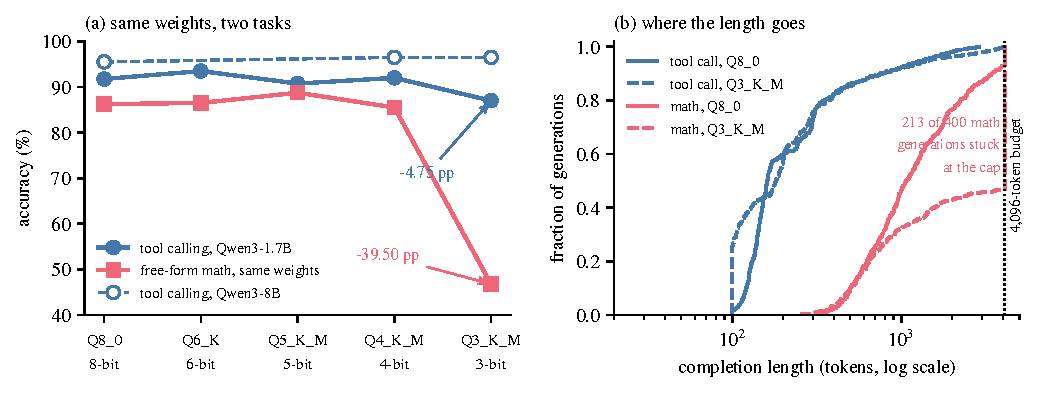
\includegraphics[width=\linewidth]{figures/fig1-ladder.pdf}
\caption{(a) Accuracy across the quantization ladder on identical weight files: tool calling on \bfcl{} and free-form mathematics on GSM8K for \qm{}, with Qwen3-8B tool calling dashed. Both floors sit at Q3\_K\_M; the free-form drop is about eight times the tool-calling drop. (b) Cumulative distribution of completion length at Q8\_0 and Q3\_K\_M for each task. Tool calls are short at both rungs, while math generations at Q3\_K\_M pile up against the 4{,}096-token budget and \qtGsmTruncThree{} of 400 never finish.}
\label{fig:ladder}
\end{figure}

\begin{table}[t]
\centering\small
\begin{tabular}{@{}llrrrlrrr@{}}
\toprule
Rung & Strict [95\% CI] & Lenient & Gap & vs.\ Q8\_0 & McNemar $p$ (Holm) & Median tokens & Truncated & Truncated, correct \\
\midrule
Q8\_0 & 86.25\% [82.5, 89.3] & 86.50\% & +0.25\,pp & baseline & & 1065 & 28 & 0 \\
Q6\_K & 86.50\% [82.8, 89.5] & 86.50\% & +0.00\,pp & $+$0.25\,pp & 1.000 (1.000) & 1102 & 32 & 0 \\
Q5\_K\_M & 88.75\% [85.3, 91.5] & 89.25\% & +0.50\,pp & $+$2.50\,pp & 0.164 (0.492) & 955 & 21 & 0 \\
Q4\_K\_M & 85.50\% [81.7, 88.6] & 85.75\% & +0.25\,pp & $-$0.75\,pp & 0.736 (1.000) & 1048 & 34 & 0 \\
Q3\_K\_M & 46.75\% [41.9, 51.6] & 46.75\% & +0.00\,pp & $-$39.50\,pp & $<$0.0001 (\textbf{$<$0.0001}) & 4096 & 213 & 29 \\
\bottomrule
\end{tabular}

\caption{The free-form control, GSM8K, $n=400$ per rung, identical weight files to Table~\ref{tab:ladder}. Extractor gap is lenient minus strict. Median tokens is the completion length; the budget was 4{,}096.}
\label{tab:gsm8k}
\end{table}

\paragraph{The extractor is not the story.} The gap between strict and lenient scoring is at most \qtGsmGapMax{} points at any rung. H3 predicted a gap of at least five points that would bound how much published free-form degradation is the parser. Once the strict extractor accepts the commitment format that reasoning models actually emit, no such gap exists. The failures at Q3\_K\_M are generations that contain no answer at all rather than answers a parser failed to find.

\paragraph{Nor is the budget.} A collapse driven by truncation could be an artefact of the 4{,}096-token cap rather than of the weights. We re-ran the \qtBudOf{} Q3\_K\_M generations that hit the cap with a budget of 16{,}384 tokens, four times the original. Of the \qtBudN{} that completed without a server error, \qtBudStillCap{} (\qtBudStillCapPct{}\%) hit the larger cap as well, and only \qtBudRecovered{} (\qtBudRecoveredPct{}\%) reached a correct answer. Given four times the room, the three-bit model mostly keeps thinking. The run-away is a property of the weights, and a larger budget converts most of the truncations into longer truncations.

\subsection{Across models}
\label{sec:models}

Table~\ref{tab:models} adds Qwen3-8B at the three rungs that matter, and at 8B there is no cliff. Q3\_K\_M scores \qtAccEightBThree{}\% against \qtAccEightBEight{}\% at Q8\_0, a difference of \qtDeltaEightBThree{} points at $p=\qtPEightBThree{}$, and Q4\_K\_M is likewise indistinguishable from the baseline. Qwen3-14B repeats the pattern: \qtAccFourteenBEight{}\% at Q8\_0, \qtAccFourteenBFour{}\% at Q4\_K\_M and \qtAccFourteenBThree{}\% at Q3\_K\_M, with the Q3\_K\_M difference at \qtDeltaFourteenBThree{} points and $p=\qtPFourteenBThree{}$. On this family the three-bit floor that binds at 1.7B has moved below the ladder by 8B and stays there at 14B, which is the direction the free-form literature reports for larger models and is now shown for the call itself at two sizes.

\begin{table}[t]
\centering\small
\begin{tabular}{@{}llrlrrlrr@{}}
\toprule
Model & Rung & $n$ & Strict [95\% CI] & vs.\ Q8\_0 & $p$ & Coerced [95\% CI] & vs.\ Q8\_0 & $p$ \\
\midrule
Qwen3-1.7B & Q8\_0 & 400 & 91.75\% [88.6, 94.1] & baseline &  & 91.75\% [88.6, 94.1] & baseline &  \\
Qwen3-1.7B & Q4\_K\_M & 400 & 92.00\% [88.9, 94.3] & $+$0.25\,pp & 1.000 & 92.00\% [88.9, 94.3] & $+$0.25\,pp & 1.000 \\
Qwen3-1.7B & Q3\_K\_M & 400 & 87.00\% [83.3, 89.9] & $-$4.75\,pp & \textbf{0.004} & 87.00\% [83.3, 89.9] & $-$4.75\,pp & \textbf{0.004} \\
\midrule
Qwen3-8B & Q8\_0 & 200 & 95.50\% [91.7, 97.6] & baseline &  & 95.50\% [91.7, 97.6] & baseline &  \\
Qwen3-8B & Q4\_K\_M & 200 & 96.50\% [93.0, 98.3] & $+$1.00\,pp & 0.625 & 96.50\% [93.0, 98.3] & $+$1.00\,pp & 0.625 \\
Qwen3-8B & Q3\_K\_M & 200 & 96.50\% [93.0, 98.3] & $+$1.00\,pp & 0.688 & 96.50\% [93.0, 98.3] & $+$1.00\,pp & 0.688 \\
\midrule
Qwen3-14B & Q8\_0 & 200 & 96.00\% [92.3, 98.0] & baseline &  & 96.00\% [92.3, 98.0] & baseline &  \\
Qwen3-14B & Q4\_K\_M & 200 & 96.00\% [92.3, 98.0] & $+$0.00\,pp & 1.000 & 96.00\% [92.3, 98.0] & $+$0.00\,pp & 1.000 \\
Qwen3-14B & Q3\_K\_M & 200 & 96.50\% [93.0, 98.3] & $+$0.50\,pp & 1.000 & 96.50\% [93.0, 98.3] & $+$0.50\,pp & 1.000 \\
\midrule
Llama-3.2-3B & Q8\_0 & 200 & 92.00\% [87.4, 95.0] & baseline &  & 93.50\% [89.2, 96.2] & baseline &  \\
Llama-3.2-3B & Q4\_K\_M & 200 & 88.00\% [82.8, 91.8] & $-$4.00\,pp & \textbf{0.021} & 91.00\% [86.2, 94.2] & $-$2.50\,pp & 0.125 \\
Llama-3.2-3B & Q3\_K\_M & 200 & 86.50\% [81.1, 90.6] & $-$5.50\,pp & \textbf{0.007} & 91.00\% [86.2, 94.2] & $-$2.50\,pp & 0.180 \\
\midrule
Llama-3.1-8B & Q8\_0 & 200 & 50.00\% [43.1, 56.9] & baseline &  & 92.00\% [87.4, 95.0] & baseline &  \\
Llama-3.1-8B & Q4\_K\_M & 200 & 63.00\% [56.1, 69.4] & $+$13.00\,pp & \textbf{$<$0.0001} & 90.50\% [85.6, 93.8] & $-$1.50\,pp & 0.453 \\
Llama-3.1-8B & Q3\_K\_M & 200 & 71.50\% [64.9, 77.3] & $+$21.50\,pp & \textbf{$<$0.0001} & 85.00\% [79.4, 89.3] & $-$7.00\,pp & \textbf{0.003} \\
\bottomrule
\end{tabular}

\caption{Tool calling across model size, \texttt{simple\_python}. Qwen3-1.7B at $n=400$; Qwen3-8B and Qwen3-14B at $n=\qtNEightB{}$. Each model is compared against its own Q8\_0.}
\label{tab:models}
\end{table}

\subsection{A second family}
\label{sec:family}

Table~\ref{tab:llama} repeats the three-rung ladder on two Llama models. The Qwen3 pattern does not transfer. Llama-3.2-3B loses \qtDropLlamaThreeBFour{} points on tool calling at Q4\_K\_M ($p=\qtPLlamaThreeBFour{}$) and \qtDropLlamaThreeBThree{} at Q3\_K\_M ($p=\qtPLlamaThreeBThree{}$), so on this model the floor is already above four bits. Its free-form accuracy falls \qtLlamaThreeBGsmDropThree{} points at Q3\_K\_M, and again the tool call is the smaller loss, but the margin between the two tasks is narrower than on Qwen3-1.7B.

Llama-3.1-8B moves the other way under the strict checker. Its Q8\_0 weights score \qtAccLlamaEightBEight{}\% on tool calling; Q4\_K\_M and Q3\_K\_M score \qtAccLlamaEightBFour{}\% and \qtAccLlamaEightBThree{}\%, both at $p<0.0001$ against Q8\_0. The failure breakdown gives the reason. Of the \qtLlamaEightBFailsEight{} Q8\_0 failures, \qtLlamaEightBTypeErrEight{} are type errors: the model names the right function and the right value but quotes the number, as in \texttt{\{"base": "10"\}}, and the AST checker rejects the type. At Q3\_K\_M, \qtLlamaEightBTypeErrThree{} of \qtLlamaEightBFailsThree{} failures are of that kind. To separate the habit from the capability we re-score every rung under a coercing checker that accepts a quoted number, list or boolean when the parsed value is what the reference holds; nothing is re-run, and the Qwen3 scores do not change because none of their failures are of this type. The coerced column of Table~\ref{tab:llama} restores the expected order: Llama-3.1-8B scores \qtLlamaEightBCoercedAccEight{}\%, \qtLlamaEightBCoercedAccFour{}\% and \qtLlamaEightBCoercedAccThree{}\% down the ladder, a \qtLlamaEightBCoercedDropThree{}-point loss at three bits, and Llama-3.2-3B scores \qtLlamaThreeBCoercedAccEight{}\%, \qtLlamaThreeBCoercedAccFour{}\% and \qtLlamaThreeBCoercedAccThree{}\%. So the compressed 8B weights write bare numbers more often, which raises the strict score, while the underlying call gets slightly worse and free-form accuracy falls \qtLlamaEightBGsmDropThree{} points at the same rung. Length plays no part in either model: GSM8K completions have a median of \qtLlamaThreeBGsmMedTokEight{} to \qtLlamaEightBGsmMedTokEight{} tokens, and at most \qtLlamaEightBGsmTruncThree{} of 400 reach the budget at any rung, so the run-away behind the Qwen3 collapse cannot occur and the free-form losses here are ordinary precision loss.

Two readings follow. The tool-calling floor is a property of the model, not of the format: four bits is safe on every Qwen3 size we measured and costs Llama-3.2-3B \qtDropLlamaThreeBFour{} points under the strict checker and \qtLlamaThreeBCoercedDropFour{} under the coercing one. And a strict schema score can move in either direction under quantization, because it measures a formatting habit as much as a capability; anyone scoring tool calls under compression should report the failure types and a coerced score beside the strict one.

\begin{table}[t]
\centering\small
\begin{tabular}{@{}llrrrrrrr@{}}
\toprule
Model & Rung & Tool acc. & vs.\ Q8\_0 & $p$ & Coerced & GSM8K strict & vs.\ Q8\_0 & $p$ \\
\midrule
Llama-3.2-3B & Q8\_0 & 92.00\% & baseline &  & 93.50\% & 84.00\% & baseline &  \\
Llama-3.2-3B & Q4\_K\_M & 88.00\% & $-$4.00\,pp & \textbf{0.021} & 91.00\% & 81.25\% & $-$2.75\,pp & 0.126 \\
Llama-3.2-3B & Q3\_K\_M & 86.50\% & $-$5.50\,pp & \textbf{0.007} & 91.00\% & 75.50\% & $-$8.50\,pp & \textbf{$<$0.0001} \\
\midrule
Llama-3.1-8B & Q8\_0 & 50.00\% & baseline &  & 94.00\% & 91.00\% & baseline &  \\
Llama-3.1-8B & Q4\_K\_M & 63.00\% & $+$13.00\,pp & \textbf{$<$0.0001} & 93.00\% & 87.75\% & $-$3.25\,pp & \textbf{0.041} \\
Llama-3.1-8B & Q3\_K\_M & 71.50\% & $+$21.50\,pp & \textbf{$<$0.0001} & 87.00\% & 83.25\% & $-$7.75\,pp & \textbf{$<$0.0001} \\
\bottomrule
\end{tabular}

\caption{The second family. Tool calling on \texttt{simple\_python}, $n=\qtNEightB{}$ per rung; GSM8K strict accuracy, $n=400$; each model against its own Q8\_0 by McNemar's exact test.}
\label{tab:llama}
\end{table}

\subsection{Harder categories}

The pre-registration predicted that multi-turn trajectories, where an error in one call corrupts the state for every call after it, would degrade at least twice as fast as single calls. They degrade far faster than that. On \bfcl{}'s \texttt{multi\_turn\_base}, $n=\qtMtN{}$, \qm{} scores \qtMtAccEight{}\% at Q8\_0, \qtMtAccFour{}\% at Q4\_K\_M and \qtMtAccThree{}\% at Q3\_K\_M. The Q4\_K\_M drop is \qtMtRelFour{}\% relative against \qtSingleRelFour{}\% for single calls at the same rung, in the predicted direction but not significant at this $n$ ($p=\qtMtPFour{}$). The Q3\_K\_M drop is \qtMtRelThree{}\% relative against \qtSingleRelThree{}\% for single calls, at $p\qtMtPThree{}$. H5 is supported at three bits by a wide margin.

The size of the multi-turn collapse follows from \S\ref{sec:freeform}. A single call is a short generation and survives three-bit weights because it ends before the length instability has room to develop. A multi-turn trajectory is many generations in sequence, each conditioned on the accumulated state, so the same per-step failure rate compounds and a single malformed call anywhere in the sequence fails the whole trajectory. The server logs show the instability reaching the call once calls are chained: at Q3\_K\_M the median generation per request is \qtMtNgenMedThree{} tokens against \qtMtNgenMedEight{} at Q8\_0, and the 90th percentile \qtMtNgenPninezeroThree{} against \qtMtNgenPninezeroEight{}. The same weights that keep a single call to \qtToolNgenMedThree{} tokens let a conditioned call run more than twice as long, and the extra length is the run-away from \S\ref{sec:freeform}, now with a schema to break. The low absolute base rate, \qtMtAccEight{}\% even at Q8\_0, is a property of the category for a 1.7B model and is why the Q4\_K\_M comparison is underpowered; it does not affect the Q3\_K\_M conclusion.

\subsection{Does the overthinking penalty transfer}

The penalty has no measurable effect. With it, \qm{} scores \qtHfourAccFour{}\% at Q4\_K\_M and \qtHfourAccThree{}\% at Q3\_K\_M, identical to the unpenalised runs to two decimals; at each rung \qtHfourLostFour{} questions flip one way and \qtHfourGainedFour{} the other. H4 predicted a loss of at least three points and there is no loss. The explanation follows from \S\ref{sec:freeform}: the penalty acts on tokens a reasoning trace emits and a tool call does not, so on a \qtToolNgenMedThree{}-token output there is almost nothing for it to act on. This agrees with the authors' own scope statement that the marker list was curated for free-form English reasoning. Both the failure they describe and the fix for it live in the reasoning trace, and the tool call contains very little of that trace.

\section{Limitations}

Three sizes of one model family and two sizes of a second, on the easiest \bfcl{} category plus one multi-turn set for Qwen3-1.7B only, on one hardware platform. The ladder is one quantization family; GPTQ, AWQ and the other research methods are deliberately out of scope, and multilingual degradation is excluded because \citet{marchisio2024multilingual} already cover it. The reproducibility control was run on two rungs rather than all five. The free-form control uses a 4{,}096-token budget; the 16{,}384-token re-run in \S\ref{sec:freeform} shows that a larger budget recovers few of the \qtGsmTruncThree{} truncated generations. The overthinking penalty is one fixed $\lambda$ rather than the authors' tuned value. Multi-turn is underpowered at $n=\qtMtN{}$ and a 17\% base rate, and was not run on Llama. A third family, and the multi-turn category on Llama, are the next additions.

\section{Conclusion}

We expected a function signature, having no slack, to be the first thing quantization breaks. On the deployed format, with no judge in the pipeline, it turned out to be the output that held up best. For \qm{} the tool-calling floor and the free-form floor sit at the same rung, between four and three bits, but the call loses \qtDropThree{} points where the mathematics loses \qtGsmDropThree{}. The difference is explained by length. Three-bit weights make the chain of thought grow past the token budget, and a call is complete long before that happens. On Qwen3-8B and Qwen3-14B there is no tool-calling cliff at any rung. On Llama the floor is elsewhere: Llama-3.2-3B loses at four bits, and Llama-3.1-8B gains at three because compression changes how it types its arguments. A fair extractor changes nothing, and a penalty designed for reasoning traces finds little to act on in a call. For anyone deploying an agent on a laptop, the practical reading is that four bits is safe on Qwen3 and not on Llama-3.2-3B, that the bit-width has to be measured on the model being shipped, and that the reasoning-length failure described in the quantization literature stays in the reasoning and does not reach the tool call.

The measurement we would most like other quantization studies to adopt is the reproducibility control in Table~\ref{tab:repeats}. Identical weights re-run three times moved by at most \qtMaxRepRange{} points. Without that figure, none of the other differences in this paper could be attributed to anything.

\section*{Reproducibility}
Every number in this paper is a macro recomputed from the raw \bfcl{} result and score files, and nothing is typed by hand. All raw generations are retained.
\begin{itemize}\setlength{\itemsep}{0pt}
\item \path{analysis/paper_numbers.py} writes \path{paper/tables/numbers.tex} and both tables from \path{runs/}.
\item \path{run_ladder.sh} rebuilds the ladder from the FP16 source and scores it; \path{run_model.sh} does the same for Qwen3-8B, Qwen3-14B and the multi-turn category.
\item \path{run_repeats.sh}, \path{run_gsm8k.sh}, \path{run_budget.sh} and \path{run_h4.sh} produce the reproducibility, free-form, budget and penalty arms.
\end{itemize}
Code, run logs, raw generations and the pre-registration are provided as an anonymized archive in the supplementary material, at the release tag the paper describes; the public repository will be linked on acceptance. The GGUF weight files are not in the archive; \path{run_ladder.sh} rebuilds them from the published FP16 checkpoint.

\section*{Broader Impact Statement}
This paper measures how a widely used compression format changes the accuracy of small language models at emitting function calls. The direct use is to let practitioners pick a bit-width for on-device agents from measurements rather than guesswork. A model that emits malformed or wrong tool calls can take real actions, so the multi-turn collapse at three bits reported in \S\ref{sec:models} is a reason to test agents at the exact quantization they ship with. We see no risk of harm arising from the paper beyond what already attaches to deploying tool-calling agents.

\bibliographystyle{tmlr}
\bibliography{refs}
\end{document}
